\subsubsection{Différence}
	\begin{itemize}
		\item Réalisation d'une requête POST via l'api REST permettant d'effectuer l'authentification dans le backend. 
		\item Différence au niveau de l'aspect graphique de la page de connection. 
		\item Connection via l'adresse Email et non le nom d'utilisateur. 
		\item Redirection automatique de l'utilisateur vers la page de connection l'ors de l'accès au site si l'utilisateur n'est pas connecter.
		\item Utilisation d'un LoginAuthenticator afin de pouvoir authentifier l'utilisateur dans le backend. 
		\item Utilisation de coockie pour préserver les informations de l'utilisateur. 
	\end{itemize}

\newpage
\subsubsection{Diagramme de séquence}
	\begin{figure*}[h!]
		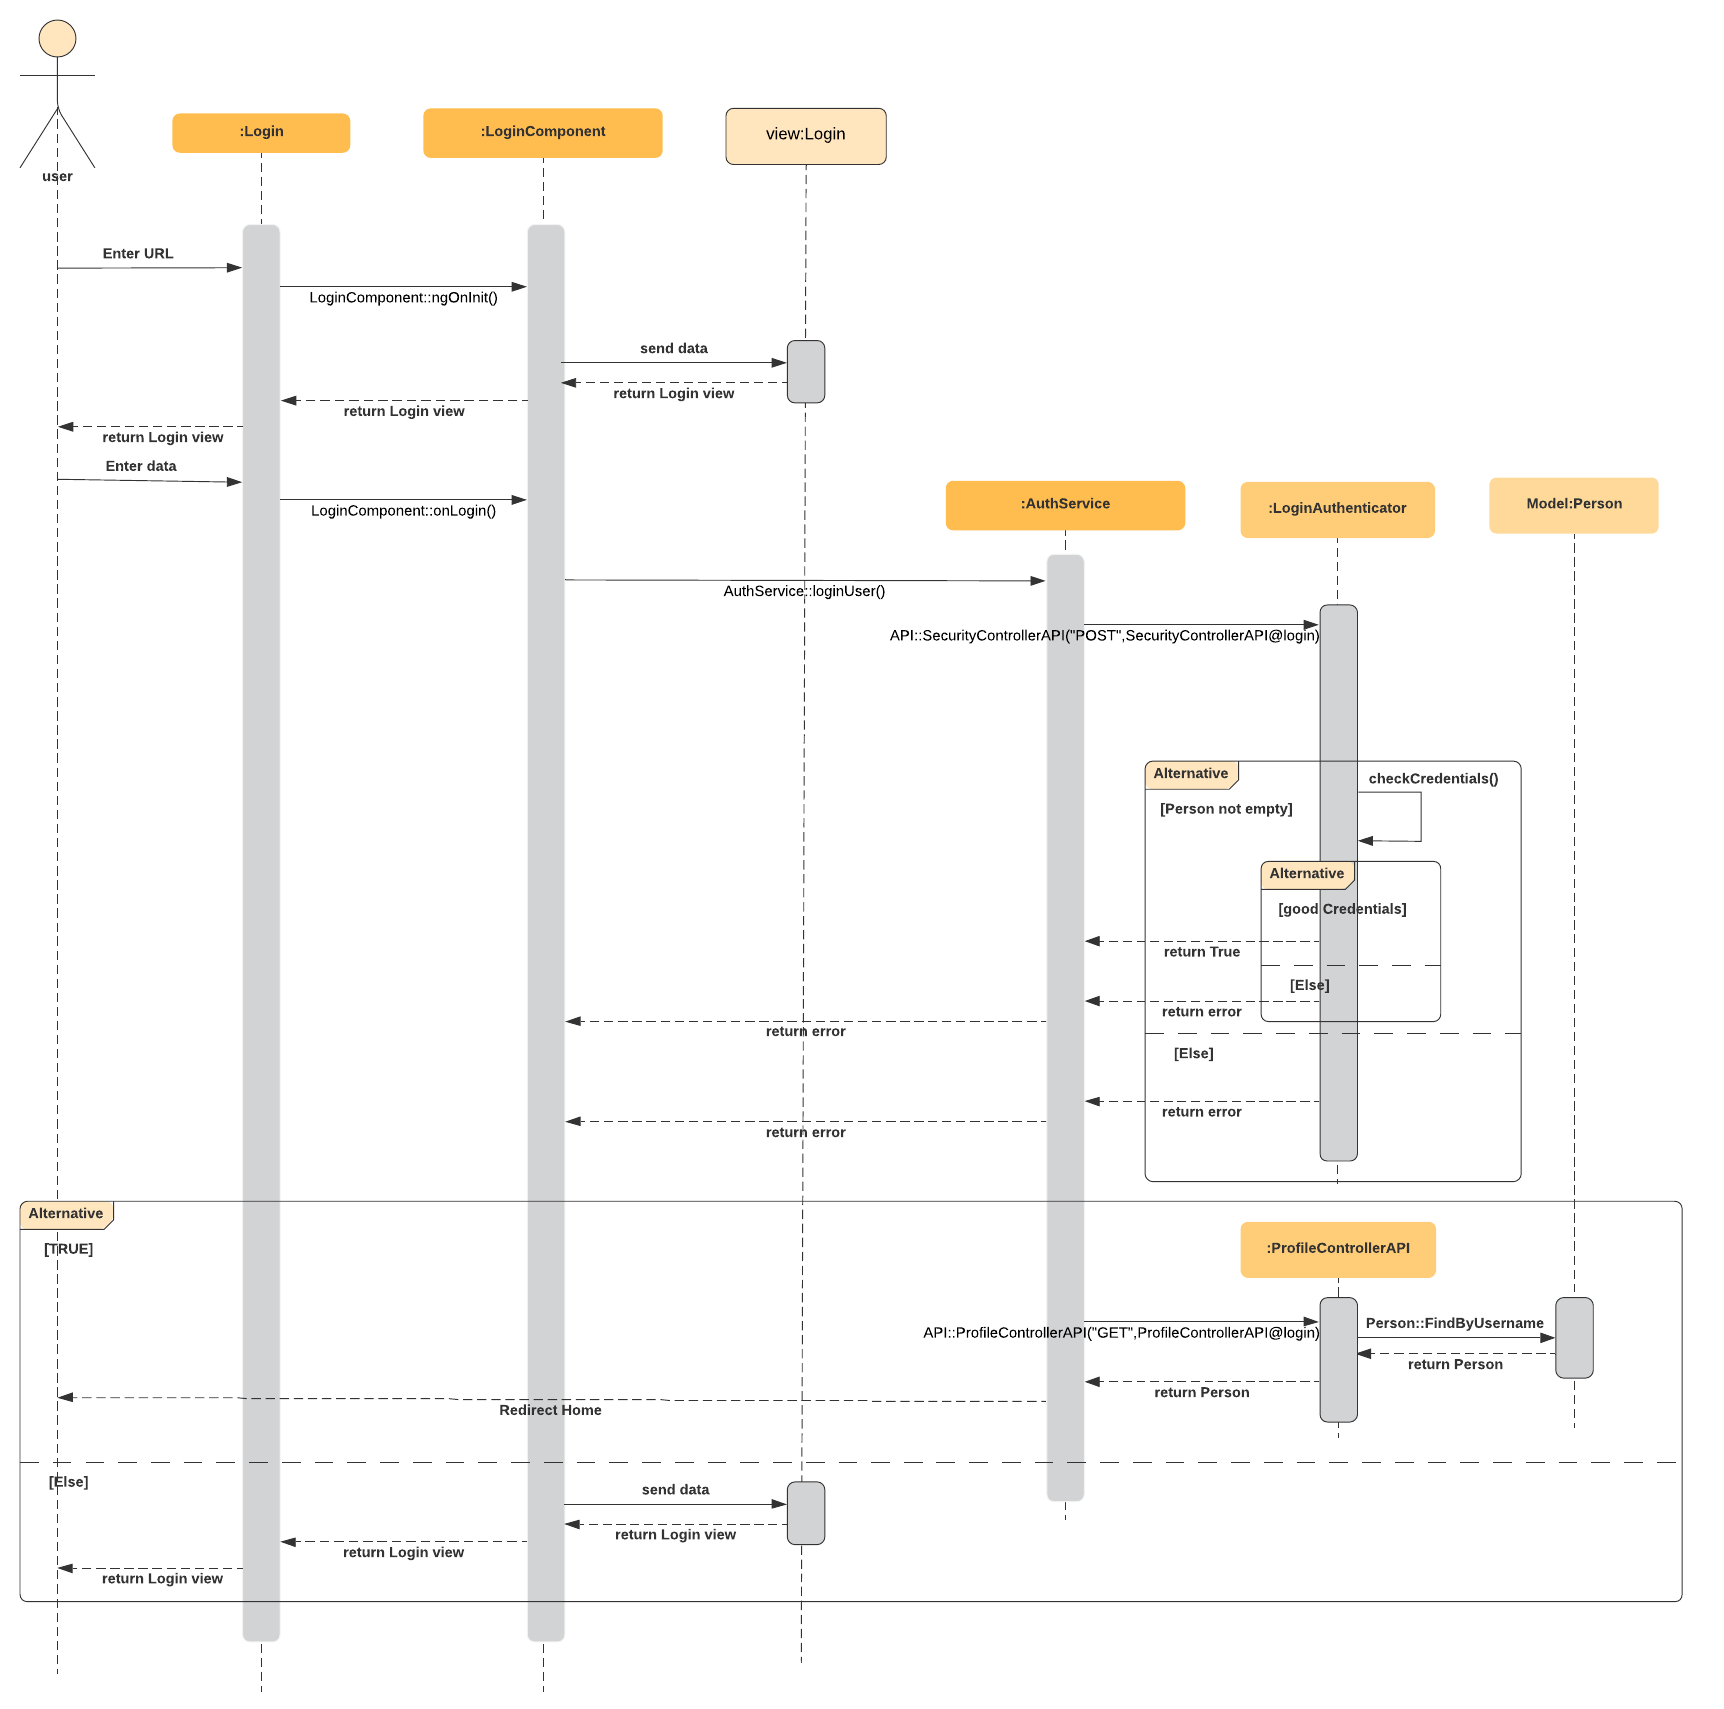
\includegraphics[width =\textwidth,center]{Diagramme/sequence-us0-angular}
		\caption{Diagramme de séquence de la connections d'un utilisateur}
	\end{figure*}

\newpage
\subsubsection{Script concernés}
	\begin{itemize}
		\item \Href{https://github.com/victorsmits/Aquabike/blob/master/frontend/src/app/service/api.service.ts}{api.service.ts}
		\item \Href{https://github.com/victorsmits/Aquabike/blob/master/frontend/src/app/service/auth.service.ts}{auth.service.ts}
		\item \Href{https://github.com/victorsmits/Aquabike/blob/master/backend/src/Controller/API/SecurityControllerAPI.php}{SecurityControllerAPI.php}
		\item \Href{https://github.com/victorsmits/Aquabike/blob/master/backend/src/Controller/API/ProfileControllerAPI.php}{ProfileControllerAPI.php}
		\item \Href{https://github.com/victorsmits/Aquabike/blob/master/frontend/src/app/login/login.component.ts}{login.component.ts}
		\item \Href{https://github.com/victorsmits/Aquabike/blob/master/frontend/src/app/login/login.component.html}{login.component.html}
		\item \Href{https://github.com/victorsmits/Aquabike/blob/master/backend/src/Entity/Person.php}{Person.php}
	\end{itemize}